% =========================================================================
% Manuscript template — Aspire Project, Study 1A
% Template only: structure mirrors paper/manuscript.md; no content.
%
% Compiles with: pdflatex -> bibtex -> pdflatex x2   (no biber needed)
%
% Venue switches (do LAST, once content is frozen):
%   * CogSci:  replace \documentclass line with the conference's cogsci class
%              (distributed with the CFP each year) and drop geometry/lineno.
%   * APA journal (e.g., PB&R): \documentclass[man,11pt]{apa7} with
%              biblatex-apa, and move Statements per journal front/back matter.
% =========================================================================
\documentclass[11pt]{article}

% ---------- packages ----------
\usepackage[margin=1in]{geometry}
\usepackage[utf8]{inputenc}
\usepackage[T1]{fontenc}
\usepackage{amsmath, amssymb, amsthm}   % equations + Proposition environment
\usepackage{booktabs}                   % tables
\usepackage{graphicx}                   % figures
\usepackage{natbib}                     % author-year citations (\citep, \citet)
\usepackage[running]{lineno}            % line numbers for review drafts
\usepackage{setspace}
\usepackage[hidelinks]{hyperref}
\usepackage{orcidlink}                  % optional: \orcidlink{0000-...}

% ---------- draft settings (remove for camera-ready) ----------
\doublespacing
\linenumbers

% ---------- theorem environments ----------
\newtheorem{proposition}{Proposition}

% ---------- helper macros (keep claims consistent with the protocol) ----------
\newcommand{\alphaw}{\ensuremath{\alpha}}                 % the mixture weight
\newcommand{\epsdual}[1]{\ensuremath{\varepsilon = 2#1}}  % response-rule dual
\newcommand{\dalpha}{\ensuremath{\Delta\alpha}}           % primary estimand
\newcommand{\repo}{\url{https://github.com/francislinlfh-lgtm/Aspire-Project}}

% ---------- metadata ----------
\title{[TITLE --- see paper/OUTLINE.md shortlist]}
\author{%
  Francis Lin\\
  {\small [Affiliation]}\\
  {\small \texttt{[email]}}%
}
\date{}   % empty for submission

% =========================================================================
\begin{document}
\maketitle

% ---------- abstract ----------
\begin{abstract}
\noindent
[Abstract --- written last. Must contain: \dalpha{} with CI; held-out CV result;
the T2 predictive-check failure.]

\medskip
\noindent\textbf{Keywords:} [perspective-taking; common ground; reference
resolution; cognitive aging; computational modeling; director task]
\end{abstract}

% ---------- 1 ----------
\section{Introduction}\label{sec:intro}
% [Scaffold paragraphs 1-6 per paper/OUTLINE.md]

% ---------- 2 ----------
\section{Model}\label{sec:model}

\subsection{A choice-level projection of the domain-mixture account}\label{sec:projection}
% [Heller Eq. 2; the reduction]
\begin{equation}\label{eq:heller}
  % P(obj \mid RE) = \alpha\, P(RE \mid obj, d{=}e)\,P(obj \mid d{=}e)
  %   + (1-\alpha)\, P(RE \mid obj, d{=}c)\,P(obj \mid d{=}c)
\end{equation}

\subsection{Hierarchy}\label{sec:hierarchy}
\begin{equation}\label{eq:hierarchy}
  % \alpha_i \sim \mathrm{Beta}(\mu(\text{age}_i)\kappa, (1-\mu(\text{age}_i))\kappa),
  % \quad e_i \sim \mathrm{Binomial}(n_i, \alpha_i)
\end{equation}
\begin{equation}\label{eq:curve}
  % \mathrm{logit}\,\mu(\text{age}) = \beta_0 + \beta_1 z + \beta_2 z^2,
  % \quad z = (\text{age} - 53)/10
\end{equation}

\subsection{Response-rule conditionality}\label{sec:equivalence}
\begin{proposition}\label{prop:equivalence}
% [matching(\alpha) and argmax+lapse(\varepsilon) likelihood-identical under
%  \epsdual{\alpha}]
\end{proposition}
\begin{proof}
% [three lines]
\end{proof}

% ---------- 3 ----------
\section{Method}\label{sec:method}
\subsection{Data}\label{sec:data}
\subsection{Cleaning and verification against published anchors}\label{sec:cleaning}
\subsection{Protocol history}\label{sec:protocol}
\subsection{Estimation and evaluation}\label{sec:estimation}
\subsection{Scope}\label{sec:scope}

% ---------- 4 ----------
\section{Results}\label{sec:results}
\subsection{Primary fit}\label{sec:fit}

% --- key-results table skeleton ---
\begin{table}[tb]
  \centering
  \caption{[Primary estimates with response-rule duals.]}
  \label{tab:main}
  \begin{tabular}{lccc}
    \toprule
    Quantity & Estimate & 95\% CI & \epsdual{\alphaw}-dual \\
    \midrule
    % \alphaw(25) &  &  &  \\
    % \alphaw(50) &  &  &  \\
    % \alphaw(75) &  &  &  \\
    % \dalpha     &  &  &  \\
    \bottomrule
  \end{tabular}
\end{table}

% --- fitted-curve figure skeleton ---
\begin{figure}[tb]
  \centering
  % 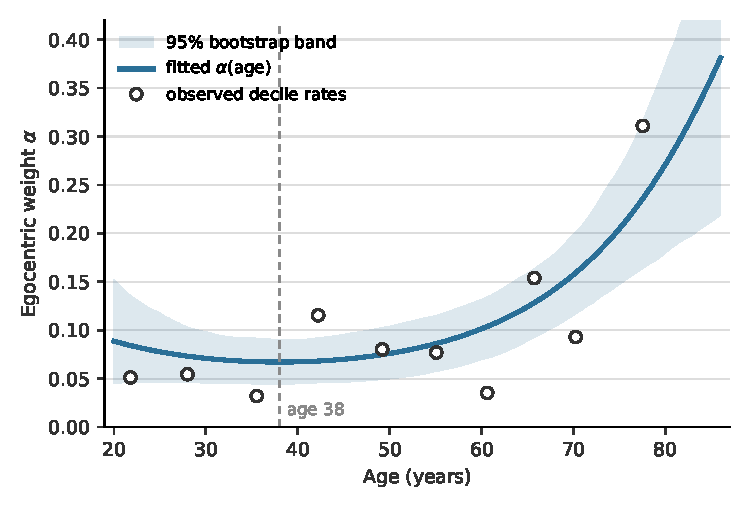
\includegraphics[width=.8\linewidth]{figures/curve.pdf}
  \caption{[Fitted \alphaw(age) with bootstrap band; observed decile rates
  overlaid; turning point marked.]}
  \label{fig:curve}
\end{figure}

\subsection{Held-out participant prediction}\label{sec:cv}
\subsection{A prespecified model failure}\label{sec:t2}
\subsection{Sensitivity analyses}\label{sec:sensitivity}

% ---------- 5 ----------
\section{Discussion}\label{sec:discussion}
% [Scaffold paragraphs 1-7 per paper/OUTLINE.md]

% ---------- statements ----------
\section*{Data and Code Availability}
% [repo + commit hashes; dataset cited, not redistributed]  \repo

\section*{AI Assistance Disclosure}
% [per venue policy]

\section*{Acknowledgments}
% [data authors; reviewer credit as appropriate]

% ---------- references ----------
\bibliographystyle{apalike}
\bibliography{references}

% ---------- appendix ----------
\appendix
\section{Protocol deviations and addenda}\label{app:addenda}
% [none, or dated addenda verbatim]

\end{document}
